\documentclass[twoside,11pt]{article}

% JMLR course template. The preprint option removes journal-specific issue data.
\usepackage[preprint]{jmlr2e}
\usepackage{booktabs}
\usepackage{multirow}
\usepackage{array}
\usepackage{enumitem}
\usepackage{microtype}
\usepackage{xcolor}
\usepackage{url}
\usepackage{lastpage}

\hypersetup{
  pdftitle={Do We Need Stratified Cross-Validation to Compare Classification Algorithms?},
  pdfauthor={Ibrahim Abd Elhadi},
  pdfsubject={Empirical Machine Learning course report},
  pdfkeywords={cross-validation, stratification, imbalanced classification, OpenML}
}

\newcommand{\regcv}{\textsc{Regular-CV}}
\newcommand{\stratcv}{\textsc{Stratified-CV}}
\newcommand{\macrof}{Macro-$F_1$}
\newcommand{\gap}{G}
\newcommand{\deltag}{\Delta G}

\jmlrheading{1}{2026}{1--\pageref{LastPage}}{August 2026}{August 2026}{EML-235975}{Ibrahim Abd Elhadi}
\ShortHeadings{Stratified Cross-Validation for Algorithm Comparison}{Abd Elhadi}
\firstpageno{1}

\begin{document}

\title{Do We Need Stratified Cross-Validation to Compare Classification Algorithms?\\
\large A Repeated 5-Fold Study Across 13 OpenML Datasets}

\author{\name Ibrahim Abd Elhadi \email matriculation no. 235975 \\
       \addr Empirical Machine Learning\\
       Supervised by JProf. Dr. Matthias Feurer and Prof. Dr. Katharina Eggensperger}

\editor{Course submission}

\maketitle

\begin{abstract}%
Cross-validation is routinely used to compare classifiers, yet the construction of the folds may influence the estimated performance and, potentially, the identity of the better algorithm. This paper studies whether stratified 5-fold cross-validation changes the comparison between Logistic Regression and a Decision Tree on 13 OpenML classification datasets. The benchmark contains between 150 and 48,842 observations and minority-class shares from 2.3\% to 44.5\%. Regular shuffled K-Fold and shuffled Stratified K-Fold are each repeated ten times with matched random seeds. Preprocessing is fitted inside every training fold, and performance is evaluated with \macrof. Across 2,600 model fits, stratification reduces the standard deviation of the smallest class share across folds by a median of 93.4\%. However, its average score effect is only $+0.00118$ for Logistic Regression and $+0.00147$ for the Decision Tree; neither effect is statistically significant. The change in the between-algorithm performance gap is also non-significant (Wilcoxon $p=0.946$), and no dataset changes its winning algorithm. Thus, stratification is an effective safeguard for fold composition, but it is neither a universal performance booster nor a determinant of the algorithm ranking in this benchmark.
\end{abstract}

\begin{keywords}
cross-validation, stratification, imbalanced classification, algorithm comparison, reproducibility, OpenML
\end{keywords}

\section{Introduction}
Model evaluation is part of the scientific claim made by an empirical machine-learning study. When a fixed train/test split is too variable or wastes scarce data, cross-validation (CV) is commonly used to estimate generalization performance. In $K$-fold CV, the observations are partitioned into $K$ mutually exclusive folds; each fold is used once for evaluation while the others are used for training. Repeating the procedure with different shuffles provides several estimates and makes the dependence on one random partition visible.

For classification, ordinary shuffled K-Fold does not constrain the class distribution in an individual fold. On an imbalanced dataset, a test fold can therefore contain very few observations from the minority class. This is especially relevant for a class-sensitive metric such as \macrof, which gives equal weight to each class. Stratified K-Fold addresses this mechanical problem by approximately preserving the global label proportions in every fold. It is often recommended as a safe default, but a more stable label composition does not automatically imply a larger, less biased, or statistically different performance estimate \citep{sklearncv}.

The scientific concern in this project is comparative rather than predictive. If two reasonable evaluation protocols reverse the ranking of two algorithms, researchers can draw incompatible conclusions from the same data. The research question is therefore:

\begin{quote}
\emph{Do we need stratified cross-validation to obtain a stable comparative conclusion between classification algorithms on balanced and imbalanced datasets?}
\end{quote}

The study compares Logistic Regression (LR), which represents a regularized linear decision boundary, and an unpruned Decision Tree (DT), which represents a nonlinear, high-variance learner. The primary outcome is the LR--DT score gap under each CV protocol. The null hypothesis $H_0$ states that the dataset-level change in this gap is centered at zero and that the protocol does not systematically change the algorithm comparison. The alternative $H_1$ states that the gap changes systematically and/or changes enough to reverse the winner on at least one dataset. Two-sided paired tests use a significance level of $\alpha=0.05$; practical relevance is evaluated from effect magnitudes and ranking reversals as well as $p$-values.

The paper makes three contributions:
\begin{itemize}[leftmargin=*,nosep]
  \item a repeated, paired evaluation on 13 heterogeneous datasets rather than a conclusion based on one example;
  \item an operational analysis of score shifts, estimate variability, fold composition, comparison-gap changes, and ranking flips; and
  \item a leakage-safe and reproducible implementation with fixed OpenML IDs, fixed random seeds, explicit software versions, and compute reporting.
\end{itemize}

\section{Background}
\subsection{Regular and stratified cross-validation}
Let $\mathcal{D}=\{(x_i,y_i)\}_{i=1}^{n}$ be a labeled dataset. In shuffled $K$-fold CV, a random permutation of $\mathcal{D}$ is partitioned into $K$ disjoint test folds. Each observation appears in exactly one test fold per repeat. The procedure aims to distribute observations evenly, but it does not constrain the distribution of $y$.

Stratified K-Fold performs the partition conditionally on the class label. For each class, its observations are distributed across folds so that the class proportions are approximately preserved. This prevents pathological splits with a missing or extremely small class, provided the number of examples is sufficient. Stratification controls only the marginal distribution of the target. It does not balance feature distributions, difficult subgroups, duplicates, groups, or temporal drift. Consequently, it is an engineering solution to one source of split variability, not a general solution to all forms of sampling bias.

\subsection{Class imbalance and the evaluation metric}
Class imbalance can interact with sample size, concept complexity, and the inductive bias of a classifier \citep{japkowicz2002}. Accuracy can conceal poor minority-class performance because the majority class dominates the count of correct predictions. This study therefore uses \macrof. For $C$ classes, class-wise precision $P_c$, and recall $R_c$, it is
\begin{equation}
F_{1,\mathrm{macro}}=\frac{1}{C}\sum_{c=1}^{C}\frac{2P_cR_c}{P_c+R_c}.
\end{equation}
Each class contributes equally, irrespective of its prevalence. When a prediction contains no positive examples for a class, the implementation uses a zero-division value of 0. This makes the metric definition explicit and avoids undefined fold results.

\subsection{Comparing algorithms across datasets}
Fold-level observations from one dataset are not independent: their training sets overlap and the same observations are reused across repeats. Treating all folds as independent would exaggerate the effective sample size. Following recommendations for multi-dataset comparisons \citep{demsar2006}, datasets are the units of the primary statistical analysis. The paired Wilcoxon signed-rank test is used because only 13 dataset-level effects are available and normality cannot be assumed. A paired $t$-test is reported as a sensitivity analysis, while effect sizes and rank reversals provide the practical interpretation.

\section{Relevant Work}
Early empirical work showed that the choice of resampling procedure affects error estimation and model selection. \citet{kohavi1995} compared cross-validation and bootstrap variants and emphasized the trade-off between bias and variance. The present study asks a narrower question: whether label-preserving fold construction, while keeping the number of folds and repeats fixed, changes an algorithm comparison.

\citet{demsar2006} developed practical guidance for statistical comparisons of classifiers over multiple datasets. Their central lesson---pairing results at the dataset level and using non-parametric procedures when appropriate---motivates the main test in this paper. The current experiment differs from broad classifier benchmarks because the two learners are fixed and the manipulated factor is the CV splitter.

The empirical infrastructure follows the reproducibility goals of OpenML \citep{vanschoren2014} and the estimator and pipeline interfaces of scikit-learn \citep{pedregosa2011}. The initial project proposal used Blood Transfusion and Iris as illustrative examples. Those two datasets suggested small differences, but they span neither the severe imbalance nor the size variation needed for a broader conclusion. The final benchmark therefore expands the design to 13 datasets, ten repeated splits, fold-local preprocessing, and dataset-level paired tests.

\section{Methodology and Experimental Setup}
\subsection{Benchmark datasets}
The datasets were fixed in the project proposal and fetched by OpenML data ID, preventing substitution with similarly named variants. Table~\ref{tab:datasets} summarizes the suite. It spans small and medium sample sizes, numeric and categorical features, binary and multiclass targets, and a wide imbalance range. Iris is the only three-class dataset; all others are binary. PC1 and Mammography are the most severe cases, with minority-class shares of 6.9\% and 2.3\%, respectively.

\begin{table}[t]
\centering
\caption{Benchmark datasets. $n$ is the number of observations, $p$ the number of input features, and ``Minority'' the smallest class share.}
\label{tab:datasets}
\small
\resizebox{\linewidth}{!}{%
\begin{tabular}{lrrrr@{\qquad}lrrrr}
\toprule
Dataset & ID & $n$ & $p$ & Minority & Dataset & ID & $n$ & $p$ & Minority \\
\midrule
Blood Transfusion & 1464 & 748 & 4 & 23.8\% & German Credit & 31 & 1,000 & 20 & 30.0\% \\
Adult & 1590 & 48,842 & 14 & 23.9\% & KC1 & 1067 & 2,109 & 21 & 15.5\% \\
QSAR Biodeg. & 1494 & 1,055 & 41 & 33.7\% & PC1 & 1068 & 1,109 & 21 & 6.9\% \\
Spambase & 44 & 4,601 & 57 & 39.4\% & ILPD & 1480 & 583 & 10 & 28.6\% \\
Iris & 61 & 150 & 4 & 33.3\% & Diabetes & 37 & 768 & 8 & 34.9\% \\
Credit Approval & 29 & 690 & 15 & 44.5\% & Mammography & 310 & 11,183 & 6 & 2.3\% \\
Phoneme & 1489 & 5,404 & 5 & 29.3\% & & & & & \\
\bottomrule
\end{tabular}
}
\end{table}

This is a deliberately heterogeneous benchmark, not a random sample of all classification tasks. Inference therefore applies to the selected suite. The breadth is nevertheless important because a single balanced dataset would not stress the property that stratification is designed to control.

\subsection{Experimental factors and models}
For every dataset, two splitters are compared:
\begin{enumerate}[leftmargin=*,nosep]
  \item \regcv: shuffled 5-fold K-Fold;
  \item \stratcv: shuffled 5-fold Stratified K-Fold.
\end{enumerate}
Both procedures are repeated ten times. Repeat $r$ uses seed $235975+r$, and the same sequence of repeat seeds is used for both protocols and algorithms. This matching removes an avoidable source of noise while preserving the intended difference in fold construction.

The classifiers are an L2-regularized LR fitted with the \texttt{lbfgs} solver and at most 2,000 iterations, and an unpruned DT. The tree's random seed is fixed to the repeat seed. No class weighting, resampling, feature selection, or hyperparameter tuning is performed. These exclusions are deliberate: they keep the splitter as the only intended experimental difference and avoid a second model-selection layer.

\subsection{Leakage-safe preprocessing}
Preprocessing is contained in a pipeline and refitted on every training fold. Numeric variables are imputed with the training-fold median and standardized. Categorical variables are imputed with the training-fold mode and one-hot encoded with unknown categories ignored. The fitted transformations are then applied to the corresponding held-out fold. This design prevents information from the test fold from influencing imputation values, scaling parameters, or the category vocabulary.

Each split is reused for LR and DT, preserving a paired comparison within a protocol. The prediction on the held-out fold is scored with \macrof. Aggregating $10\times5=50$ fold scores produces one mean per dataset--protocol--algorithm combination. With 13 datasets, two protocols, two algorithms, ten repeats, and five folds, the full experiment contains
\begin{equation}
13\times2\times2\times10\times5=2{,}600
\end{equation}
model fits.

\subsection{Outcomes and hypothesis tests}
For dataset $d$ and protocol $p$, define the algorithm-comparison gap
\begin{equation}
\gap_{d,p}=\overline{F}_{1,d,p,\mathrm{LR}}-\overline{F}_{1,d,p,\mathrm{DT}},
\qquad
\deltag_d=\gap_{d,\mathrm{Stratified}}-\gap_{d,\mathrm{Regular}}.
\end{equation}
A positive gap favors LR, a negative gap favors DT, and a ranking flip occurs when the signs under the two protocols differ. The primary test applies a two-sided Wilcoxon signed-rank test to the 13 values of $\deltag_d$. A paired $t$-test is reported as a sensitivity check.

Secondary outcomes are: (i) the stratified-minus-regular mean \macrof separately for each model; (ii) the standard deviation of the ten repeat-level mean scores, analyzed over 26 dataset--algorithm pairs; (iii) the standard deviation of the smallest class share across the five test folds; and (iv) the Spearman association between dataset minority share and the average protocol score effect. These outcomes distinguish a mechanical improvement in fold construction from a performance change.

\section{Implementation Details}
The experiment uses Python 3.12.13, scikit-learn 1.8.0, NumPy 2.3.5, pandas 2.2.3, and SciPy 1.17.0. OpenML provides the fixed dataset identities and automated retrieval. scikit-learn implements the splitters, preprocessing pipelines, estimators, and metric; pandas and NumPy organize the results; SciPy performs the paired Wilcoxon, paired $t$, and Spearman tests.

Independent dataset--repeat--protocol tasks are executed with four parallel workers. Within a task, the same folds are used for both algorithms. The machine exposes nine logical CPUs and runs x86\_64 Linux. The complete run takes 105.8 seconds of wall-clock time; summed fit-and-score time is 376.2 seconds. The difference reflects parallel execution and the fact that the summed time counts concurrent work separately.

Reproducibility controls include fixed OpenML IDs, a documented base seed, matched seeds across protocols, fold-local preprocessing, explicit model configurations, and retention of fold-level scores and timings. The complete reproduction script, reported result tables, figure-generation code, environment requirements, and JMLR source are available at \url{https://github.com/ibrahem2001ab/stratified-cv-comparison}. The repository README documents the commands for rerunning the 2,600 model fits and rebuilding this paper.

\section{Results}
\subsection{Stratification stabilizes fold composition}
The direct effect of stratification is large and consistent: the standard deviation of the smallest class share across the five test folds falls by a median of 93.4\% across datasets. German Credit and Iris have identical smallest-class shares in all five stratified test folds, while Mammography is nearly exact despite its 2.3\% minority class. This confirms that the implementation behaves as intended and that the selected benchmark includes conditions in which unconstrained splitting can visibly change test-fold composition.

The class-balance range of the benchmark is shown in Figure~\ref{fig:imbalance}. The figure is descriptive rather than inferential: it identifies the stress cases for which a class-preserving splitter has the clearest mechanical motivation.

\begin{figure}[t]
\centering
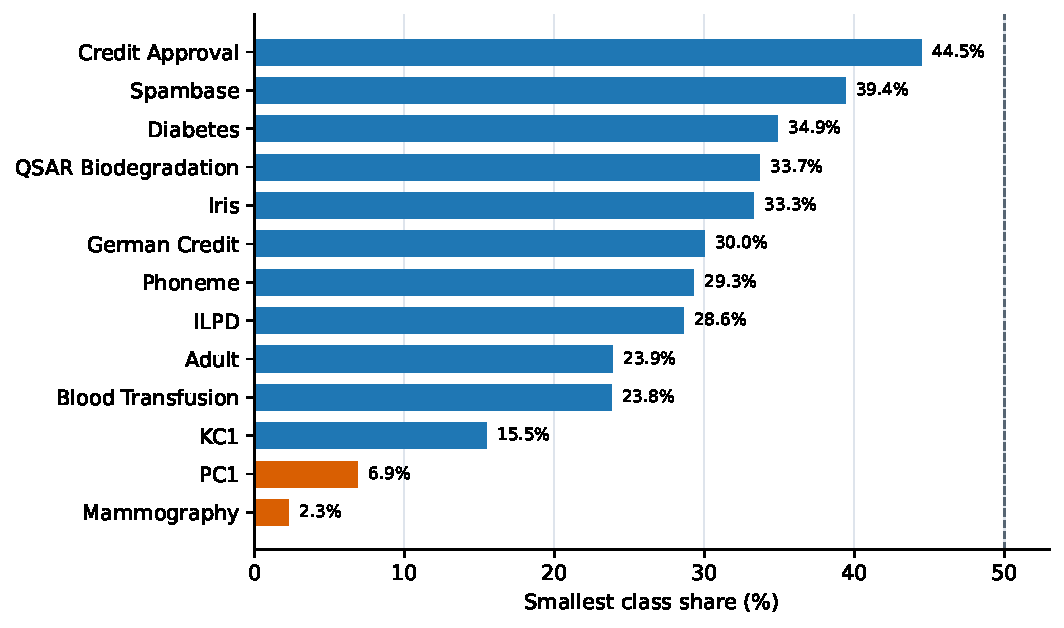
\includegraphics[width=0.88\linewidth]{figures/dataset_imbalance.pdf}
\caption{Smallest class share for the 13 OpenML datasets. The dashed line marks the balanced 50\% value for binary data; Iris is a balanced three-class dataset at 33.3\%.}
\label{fig:imbalance}
\end{figure}

\subsection{Mean score effects are small}
Table~\ref{tab:tests} reports the paired statistical tests. The average stratified-minus-regular effect is $+0.00118$ for LR and $+0.00147$ for DT. Neither the Wilcoxon test nor the paired $t$-test rejects a zero dataset-level effect. Effects do not point consistently in one direction: the largest gains are $+0.0110$ for LR on PC1 and $+0.0116$ for DT on QSAR Biodegradation, while the largest loss is $-0.0101$ for DT on Mammography. Thus, stabilizing class allocation does not produce a uniform increase in \macrof.

\begin{table}[t]
\centering
\caption{Paired effects of \stratcv minus \regcv. Score tests use 13 datasets. The variability test uses 26 dataset--algorithm pairs.}
\label{tab:tests}
\small
\begin{tabular}{lrrrr}
\toprule
Outcome & Mean & Median & Wilcoxon $p$ & Paired $t$ $p$ \\
\midrule
LR mean \macrof & $+0.00118$ & $+0.00033$ & 0.635 & 0.323 \\
DT mean \macrof & $+0.00147$ & $+0.00127$ & 0.414 & 0.437 \\
Repeat-to-repeat score SD & $-0.00094$ & $-0.00015$ & 0.247 & 0.147 \\
\bottomrule
\end{tabular}
\end{table}

The repeat-to-repeat standard deviation decreases by only 0.00094 on average and 0.00015 at the median. Its Wilcoxon $p$-value is 0.247. Therefore, a more predictable label share within a fold should not be conflated with a reliably lower variability of the final repeated-CV score.

\subsection{The algorithm ranking is unchanged}
Table~\ref{tab:gaps} presents the primary outcome. Seven datasets favor LR under both protocols, and six favor DT under both. None of the 13 signs changes. Figure~\ref{fig:gaps} visualizes the same result: every dataset stays in a quadrant that represents the same winner under regular and stratified CV.

\begin{figure}[t]
\centering
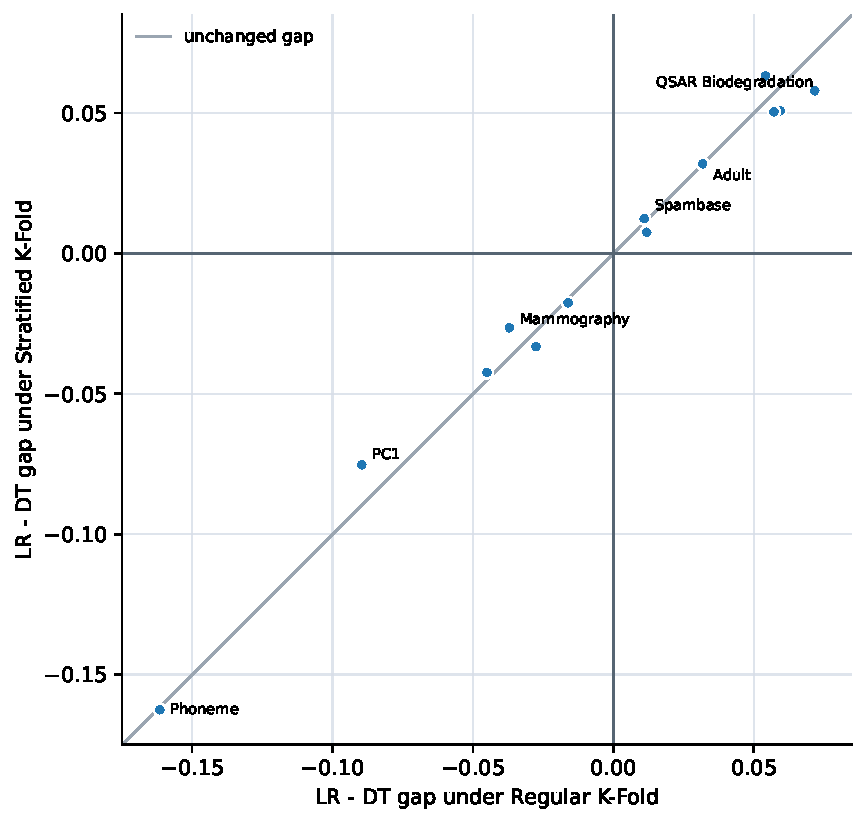
\includegraphics[width=0.78\linewidth]{figures/algorithm_gaps.pdf}
\caption{LR--DT \macrof gap under regular and stratified 5-fold CV. Positive values favor LR; negative values favor DT. A ranking flip would fall in an off-diagonal quadrant. All points remain in a same-winner quadrant.}
\label{fig:gaps}
\end{figure}

Across datasets, $\deltag$ has mean $-0.00029$, median $-0.00094$, and median absolute magnitude $0.00568$. The primary two-sided Wilcoxon signed-rank test does not reject $H_0$ ($W=44$, $p=0.946$), and the paired $t$-test agrees ($p=0.898$). The largest absolute gap change is 0.0143 on PC1; the gap remains negative, so DT still ranks higher. Numerically different estimates therefore do not imply a substantively different comparison.

An exploratory Spearman test finds no association between minority-class share and the mean protocol score effect across the two algorithms ($\rho=0.082$, $p=0.789$). Within this suite, more severe imbalance does not imply a larger score gain from stratification. The test has low power with 13 observations and should not be interpreted as proof that no relationship exists in a broader population.

\begin{table}[t]
\centering
\caption{Algorithm-comparison gaps $\gap=\overline{F}_{1,\mathrm{LR}}-\overline{F}_{1,\mathrm{DT}}$. Positive values favor LR. $\deltag$ is stratified minus regular.}
\label{tab:gaps}
\small
\resizebox{\linewidth}{!}{%
\begin{tabular}{lrrr@{\qquad}lrrr}
\toprule
Dataset & Regular & Stratified & $\deltag$ & Dataset & Regular & Stratified & $\deltag$ \\
\midrule
Adult & +.0318 & +.0319 & +.0001 & ILPD & -.0161 & -.0176 & -.0014 \\
Blood Transfusion & -.0450 & -.0424 & +.0026 & Iris & +.0119 & +.0075 & -.0044 \\
Credit Approval & +.0572 & +.0504 & -.0067 & KC1 & -.0275 & -.0332 & -.0057 \\
Diabetes & +.0542 & +.0632 & +.0089 & Mammography & -.0370 & -.0265 & +.0105 \\
German Credit & +.0594 & +.0508 & -.0086 & PC1 & -.0896 & -.0753 & +.0143 \\
Phoneme & -.1615 & -.1625 & -.0009 & QSAR Biodeg. & +.0717 & +.0579 & -.0138 \\
Spambase & +.0110 & +.0124 & +.0014 & & & & \\
\bottomrule
\end{tabular}
}
\end{table}

\section{Discussion}
The evidence separates two meanings of ``stability.'' First, fold-composition stability improves sharply: stratification makes the proportion of the smallest class predictable. Second, inferential stability---the variability and central value of the performance comparison---changes little. These findings are compatible because label prevalence is only one determinant of a fold's difficulty. Conditional feature distributions, rare subgroups, noisy labels, duplicates, and decision-boundary geometry remain uncontrolled.

For the benchmark studied here, the primary scientific conclusion is stable. Stratification changes some numeric estimates by roughly one \macrof percentage point, but the LR--DT gap remains on the same side of zero for every dataset. The absence of a ranking reversal is more directly relevant to the research question than a small change in one model's isolated score.

The result does not justify abandoning stratification. A class-preserving splitter is a low-cost safeguard when observations are exchangeable and the target is imbalanced. It reduces the risk of folds with a sparse or absent class and makes each fold more representative with respect to the target marginal. The appropriate recommendation is therefore to use stratification by default in ordinary imbalanced classification, while describing it as a protection against pathological label allocation rather than as a performance-improvement method.

The choice of splitter must still respect the data-generating process. Grouped observations require group-aware splitting to prevent leakage, and temporally ordered data require time-aware evaluation. Ordinary stratification cannot repair a protocol that breaks those structural constraints.

\section{AI Usage Declaration}
Generative AI tools were used to assist with code scaffolding, LaTeX formatting, language editing, and visual quality checks. Automated tools also supported repetitive data processing, experiment execution, aggregation, and chart generation. The research question, dataset list, algorithms, evaluation metric, experimental constraints, interpretation of statistical results, and final claims were reviewed by the author. AI-generated text and code were checked against the recorded numerical outputs; no AI system was treated as an empirical source. This assistance made it easier to learn how to express a paired multi-dataset experiment as a reproducible pipeline and how to distinguish fold-composition stability from performance stability.

\section{Limitations}
The conclusions are conditional on two untuned algorithms. Ensembles, calibrated models, class-weighted estimators, and tuned pipelines may respond differently to the split protocol. Similarly, \macrof emphasizes equal class contribution; ROC-AUC, PR-AUC, expected cost, calibration error, or application-specific utility could produce another pattern.

The 13 OpenML datasets are heterogeneous but were not sampled randomly from a defined population of tasks. Dataset-level statistical inference therefore summarizes this benchmark rather than establishing a universal law. Ten repeats provide a useful compact analysis, but problems with extremely few minority observations may require more repeats or repeated holdout designs.

Finally, the benchmark contains no grouped or time-dependent task. The recommendation applies only when observations can be treated as exchangeable. In applications with patients, users, machines, locations, or chronological drift, respecting group and temporal boundaries takes priority over ordinary label stratification.

\section{Conclusion and Future Work}
Under repeated shuffled 5-fold CV on the 13 specified OpenML datasets, stratification is not required to preserve the comparative conclusion between LR and DT. No dataset changes its winning algorithm, and the dataset-level change in the comparison gap is non-significant ($p=0.946$). The null hypothesis is therefore not rejected.

Stratification nevertheless has a clear operational benefit: it reduces fold-to-fold class-composition variability by a median of 93.4\%. The practical conclusion is concise: stratify for robustness when samples are exchangeable, but compare algorithms using repeated, paired evidence and do not present stratification as a guarantee of higher expected performance.

Future work should test additional classifiers and tuned pipelines, include metrics such as PR-AUC and calibration error, increase the number of datasets and repeats, and study splitters that combine label balance with group or temporal constraints. A particularly useful extension would analyze whether stratification matters more for model-selection decisions than for fixed-model comparisons.

\vskip 0.2in
\bibliography{references}

\end{document}
